% ── Appendix A — persistence of the sparse-VAR contagion links ────────────────
\section*{Appendix A --- Are the contagion links stationary?}

By doing the same methodology as in Part.~\ref{recurrence_var}, we can check if
the VAR coefficients are stationary. In other words, if the stock $i$ is
influenced by the stock $j$ at a certain lag for a certain period, will this
influence link still be true at another period?

To answer this, the series ($N = 146$ assets) is split into
$n_{\mathrm{chunks}} \in \{4, 10, 30\}$ consecutive chunks, and a sparse lagged
VAR (lag $= 13$, one trading day) is re-fitted on each chunk, keeping as
predictors only the pairs whose lagged correlation $|C_{ij}|$ exceeds the
quantile $q \in \{0.80, 0.90, 0.95\}$. Each ordered pair $(i,j)$ is then
characterised by its \emph{activation frequency} $F_{ij}$, the fraction of
chunks in which the link is selected. If the influence links were stationary,
the distribution of $F$ should be strongly bimodal: a core of links active in
almost every chunk, and the rest almost never. Figure~\ref{fig:A1} shows the
opposite: for every $(n_{\mathrm{chunks}}, q)$, the observed distribution of $F$
(red) is essentially indistinguishable from the one obtained if each chunk drew
its active links \emph{at random}, $F \sim \mathrm{Bin}(n_{\mathrm{chunks}},
p_{\mathrm{sel}})/n_{\mathrm{chunks}}$ (blue). At $n_{\mathrm{chunks}} = 30$,
not a single link remains active in more than half of the sub-periods. The only
significant excess over chance is marginal: $73$ links with $F \ge 0.5$ versus
$35$ expected at $n_{\mathrm{chunks}} = 10$, $q = 0.90$, i.e.\ ${\sim}0.2\%$ of
the $21\,316$ ordered pairs, concentrated on a few same-sector pairs
(META--AMZN, HD--LOW, GOOG--META, LRCX--INTC).

The interpretation of the previous sections must therefore be nuanced: the
assets carrying the strongest contagion links over one period are not
necessarily the same ones a few months later --- the identity of the top links
is redrawn almost entirely from one period to the next. For this reason, the
graphs built by keeping only the strongest links still make sense, but only as
\emph{snapshots} of the contagion structure of a given period (and the rare
links that do recur are precisely the intra-sector pairs they display); they
should not be read as a permanent map of who contaminates whom. Only the
statistical properties of the network --- degree structure, spectral radius,
communities --- are stable enough to support conclusions across periods.

\begin{figure}[t]
  \centering
  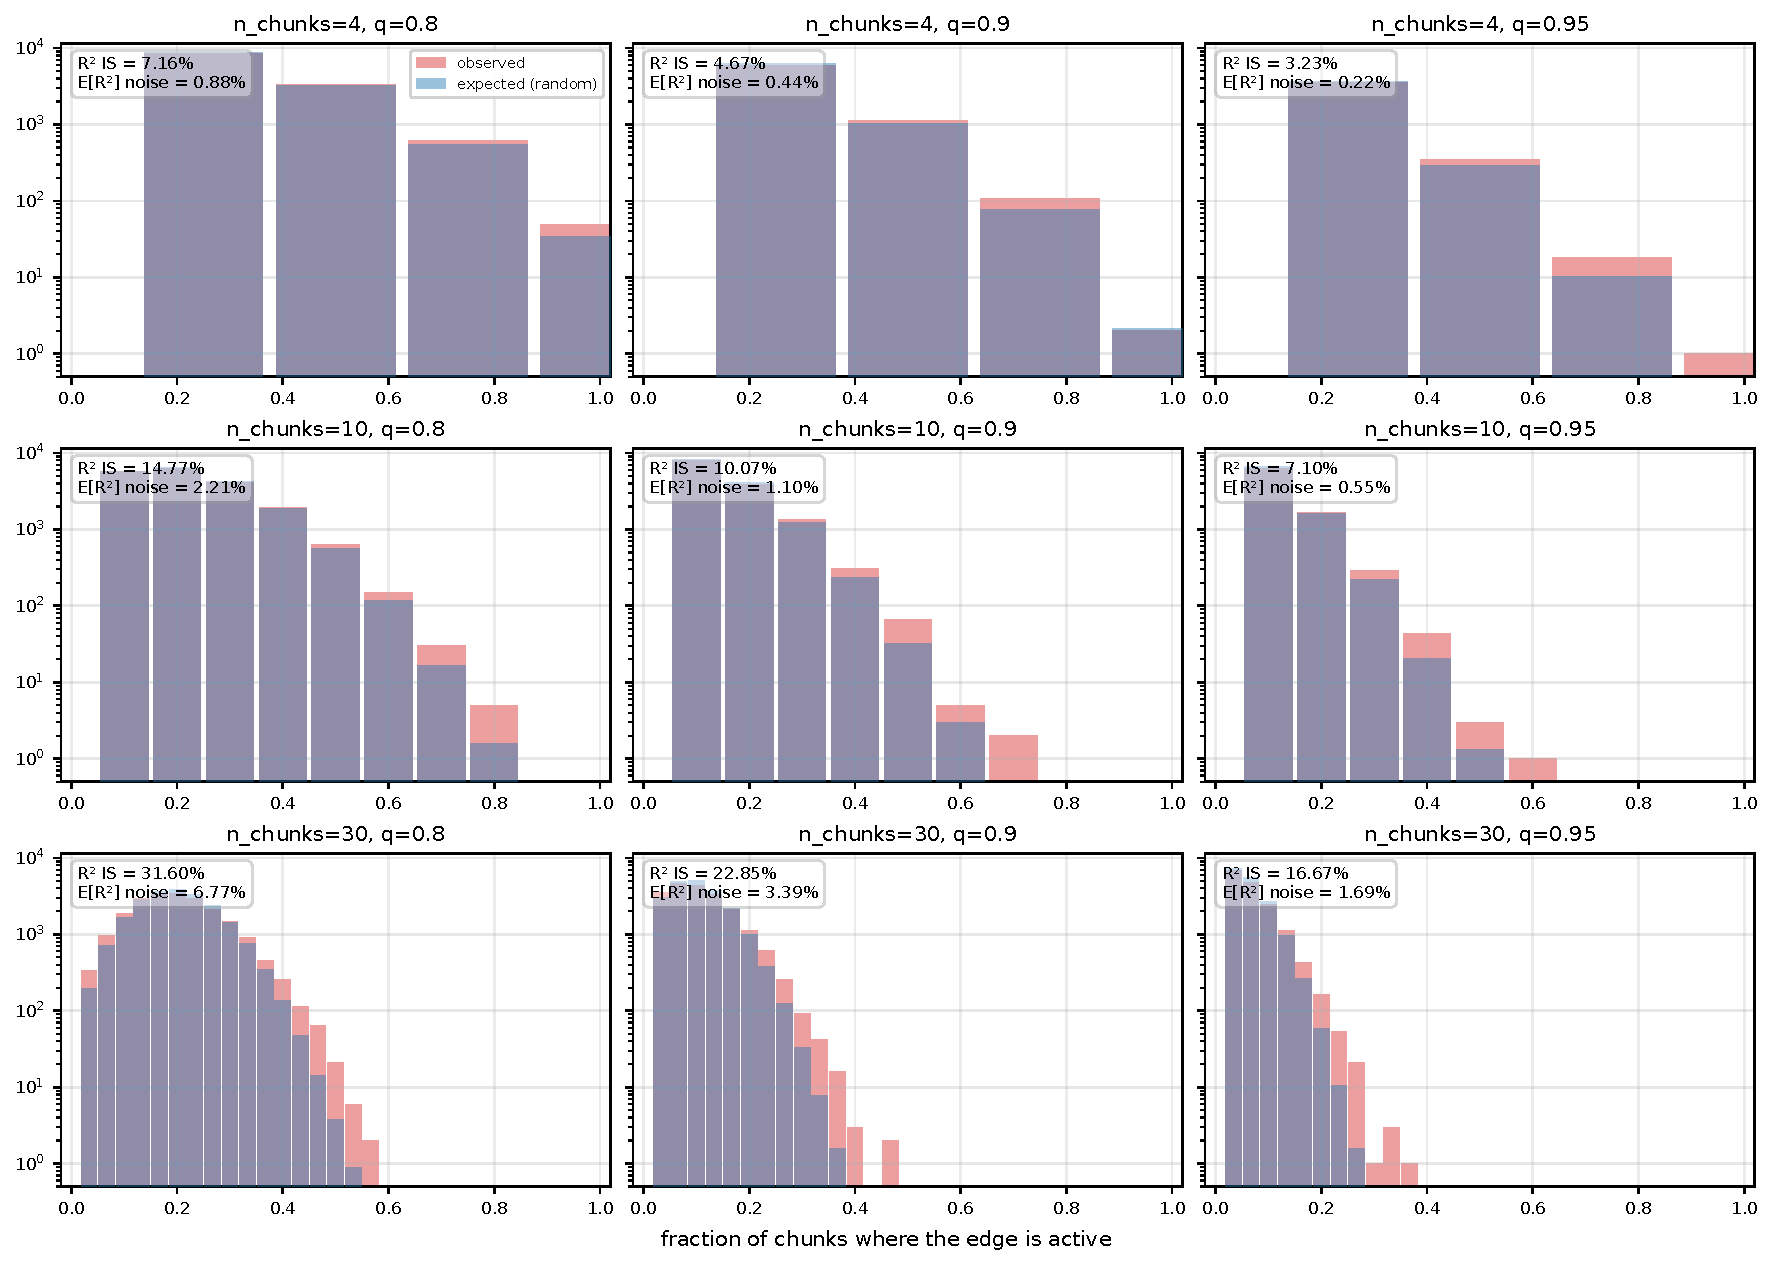
\includegraphics[width=\textwidth]{Fig/rapport/fig_A1_sparse_var_activation.pdf}
  \caption{Sparse VAR: distribution of the link activation frequency $F$ per
  $(n_{\mathrm{chunks}}, q)$, log scale. Red: observed counts; blue: counts
  expected under pure chance ($F \sim \mathrm{Bin}(n_{\mathrm{chunks}},
  p_{\mathrm{sel}})/n_{\mathrm{chunks}}$). Each panel also reports the mean
  in-sample $R^2$ and its white-noise expectation $\mathbb{E}[R^2] = k/(n-1)$.
  The observed activation frequencies follow the random-turnover prediction:
  the individual contagion links do not persist across sub-periods.}
  \label{fig:A1}
\end{figure}
